\documentclass[mathserif]{beamer}

\usetheme{Warsaw}

\usepackage[utf8x]{inputenc} 
\usepackage[spanish]{babel} %idioma
\usepackage{ucs}
\usepackage{amsmath, amssymb}
\usepackage{dsfont}
\usepackage{graphics}
\usepackage{cases}
\usepackage{graphicx}
\usepackage{pgf}
\usepackage{epsfig}
\usepackage{amssymb}
\usepackage{amstext}
\usepackage[ruled,vlined,lined]{algorithm2e}
\usepackage{amsmath}
\usepackage{epic}
\usepackage{fontenc}
\usepackage{palatino, url, multicol}
%\algsetup{indent=2em}
\newcommand{\factorial}{\ensuremath{\mbox{\sc Factorial}}}
\newcommand{\BIGOP}[1]{\mathop{\mathchoice%
{\raise-0.22em\hbox{\huge $#1$}}%
{\raise-0.05em\hbox{\Large $#1$}}{\hbox{\large $#1$}}{#1}}}
\newcommand{\bigtimes}{\BIGOP{\times}}

\vspace{-0.5cm}
\date{\today}
\logo{
\includegraphics[height=1cm]{pics/logo-fcfm.jpg}}
\title{Procesamiento de Texto y Modelo Vectorial}
\author[F.Bravo-Marquez]{Felipe Bravo Márquez}

\begin{document}
\begin{frame}
\titlepage
\end{frame}

\begin{frame}\frametitle{Motivación}


  \begin{itemize}
   \item ¿Cómo recupera un buscador como Google o Yahoo! documentos relevantes a partir de una consulta enviada?
   \item ¿Cómo puede procesar una empresa los reclamos que le dejan sus usuarios en sus portales Web?
   \item ¿Cómo podemos agrupar los comentarios emitidos en un foro y analizar las opiniones de la gente?
  \end{itemize}



Para resolver esos problemas, hay que estudiar las siguientes áreas del conocimiento:

\begin{itemize}
 \item \emph{Recuperación de Información}: Ciencia encargada de la búsqueda de información en documentos.
 \item \emph{Text Mining}: Extracción de conocimiento a partir del texto.
\end{itemize}



\end{frame}

\begin{frame}\frametitle{Tokens y Tipos}
{\footnotesize
Dado un documento $d$, se llama como \emph{tokenización} a la tarea de separar el texto por palabras llamados \emph{tokens}, además se pueden borrar caracteres especiales, como la puntación y convertir los caracteres a minúsculas~\cite{manning2008}. 

\begin{block}{Ejemplo}
Input: Además de inscribir Web Mining, inscribí Data Mining.\\
Tokens: [además] [de] [inscribir] [web] [mining] [inscribí] [data] [mining]
\end{block}

Se define como un \emph{tipo} como una clase de \emph{token} que contiene una única secuencia de caracteres.
Se obtienen identificando los tokens iguales dentro del documento.

\begin{block}{Tipos}
Tipos: [además] [data] [de] [inscribí] [inscribir] [mining] [web]   \\
\center{\textit{El token \emph{mining} estaba repetido}}
\end{block}



 }
\end{frame}

\begin{frame}\frametitle{Extracción del Vocabulario de términos [1]}
\footnotesize{

Un \emph{término} es un \emph{tipo} normalizado. Se llama vocabulario $V$, al conjunto de términos de una colección de documentos $D$.
 
\begin{block}{Borrado de Stopwords}
Para reducir la dimensión del vocabulario y eliminar términos que no aportan información, se eliminan los términos que aparecen
con mucha frecuencia en la mayoría de los documentos(stopwords). Como artículos, pronombres,  preposiciones y conjunciones. \\
Ejemplo: [el, la , ellos, ellas,  nosotros, un, una , de, con , a , además, ya, y, muy, otro, cuando, cuanto ]. 
\end{block}

\begin{block}{Stemming}
Proceso donde se transforman los términos a su raíz para reducir la dimensión del vocabulario. Se realiza en base a un conjunto de reglas de reducción de palabras. Ejemplo: Algoritmo de Porter.

\begin{figure}[h!]
	\centering
	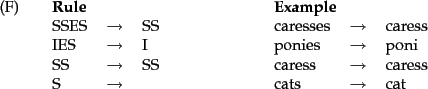
\includegraphics[scale=0.45]{pics/porter.png}
\end{figure}


\end{block}
}
 
\end{frame}

\begin{frame}\frametitle{Extracción del Vocabulario de términos [2]}
\footnotesize{
 
\begin{block}{Lematización}
\begin{itemize}
 \item Es otra estrategia para llevar las palabras a su raíz. Realiza un análisis morfológico por medio de diccionarios de referencia para crear clases de equivalencia entre \emph{tipos}. 
\item Por ejemplo para el token \emph{saw}, una regla de stemming podría construir un término \emph{s}, mientras que mediante lematización un diccionario nos entregaría \emph{see}. 

\end{itemize}
\end{block}

Eliminando las stopwords y haciendo uso de stemming, el vocabulario del documento $d$ queda de la siguiente forma:

\begin{table}
\centering
\begin{tabular}{c|c}
\hline
termId & value \\ 
\hline
t1 & data \\ 
t2 & inscrib \\ 
t3 & mining \\ 
t4 & web \\ 
\hline
\end{tabular}
\end{table}

}
\end{frame}



\begin{frame}\frametitle{Ley de Zipf [1]}
\footnotesize{
\begin{itemize}
 \item La ley de Zipf, propuesta por \emph{George Kingsley Zipf} en \cite{zipf1935}, se usa para el análisis de frecuencia de aparición de términos dentro de una colección de documentos. 
\item Dice que la frecuencia $f$ de aparición de un término en una colección es inversamente proporcional a su ranking $r$ en una tabla ordenada de frecuencias.
\begin{equation}
	f = \frac{cf}{r^{\beta}}
\end{equation}
\item Donde $cf$ es una constante dependiente de la colección  y $\beta > 0$ modela la razón de decaimiento.
\item Si $\beta = 1$, entonces $f$ sigue exactamente la ley de Zipf, si no se dice que sigue una distribución Zipf-like. A mayor $\beta$ menor es la calidad del lenguaje en los documentos. 

\item La ley se relaciona con el principio de mínimo esfuerzo. Usamos muchas veces unas pocas palabras para escribir las ideas.

\end{itemize}


}
 
\end{frame}


\begin{frame}\frametitle{Ley de Zipf [2]}
\footnotesize{

\begin{figure}[h!]
	\centering
	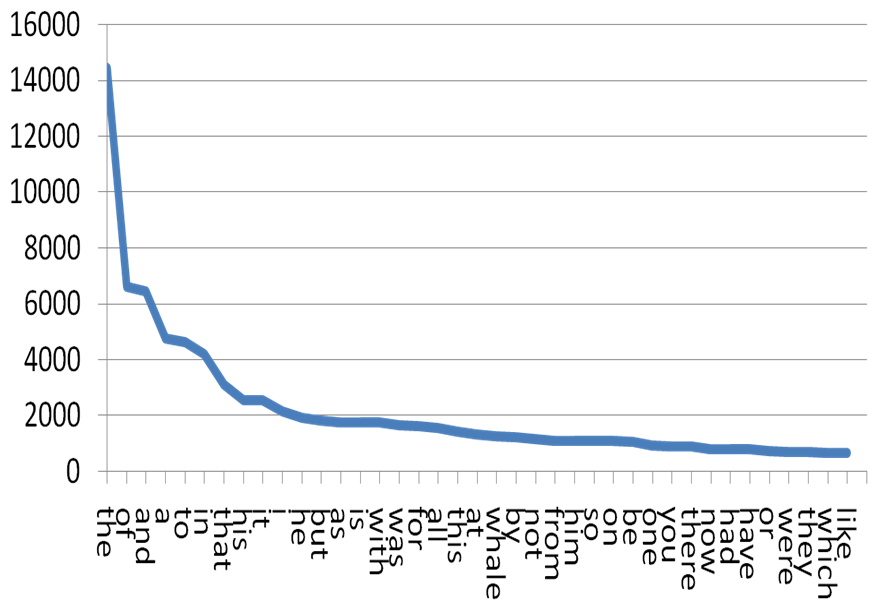
\includegraphics[scale=0.5]{pics/zipf1.png}
	\caption{Ley de Zipf}
\end{figure}
\begin{itemize}
 \item Si se realiza un gráfico $log-log$, se obtiene una recta de pendiente  $-\beta^{-1}$.
 \item Los términos más frecuentes se pueden usar para crear la lista de \emph{stopwords}. 
\end{itemize}
}



 
\end{frame}

\begin{frame}\frametitle{Lista de Posteo e Índice Invertido}
{\footnotesize Sea $D$ una colección de documentos y $V$ el vocabulario de todos los términos extraídos de la colección:

\begin{itemize}
 \item La lista de posteo de un término, es la lista de todos los documentos en los que aparece al menos una vez.
 \item Un índice invertido en una estructura de datos de diccionario que mapea cada término $t_{i} \in V$ a su lista de posteo. 
 \begin{displaymath}
  <term> \rightarrow <docId>^*
 \end{displaymath}

\end{itemize}

\begin{figure}[h!]
	\centering
	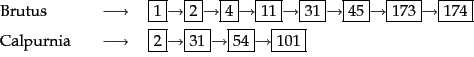
\includegraphics[scale=0.6]{pics/invFile.png}
	\caption{ Índice Invertido}
\end{figure}



}
\end{frame}



\begin{frame}\frametitle{Motor de Búsqueda [1]}


{\footnotesize
  Un motor de búsqueda es un sistema de recuperación de información diseñado para la búsqueda de información en la Web \cite{libroweb2008}. Sus componentes básicos son:


\begin{block}


\begin{itemize}
\item Crawler: Un robot que navega  la Web según una estrategia definida. Generalmente comienza navegando por un conjunto de páginas semilla (seeds) y continua navegando por sus hipervínculos.
\item Indexador: Encargado de mantener un índice invertido con el contenido de las páginas recorridas por el Crawler.
\item Máquina de consultas: Encargado de procesar las  consultas y buscar en el índice los documentos  con mayor similitud a ella.
\item Función de ranking: Es la función que tiene la máquina de consulta para rankear los documentos indexados en la colección por relevancia para una consulta.
\item Interfaz: Interactúa con el usuario, recibe la consulta como entrada y retorna los documentos rankeados por similitud.
 
\end{itemize}

\end{block}
}

\end{frame}


\begin{frame}\frametitle{Motor de Búsqueda [2]}

\begin{figure}[h!]
	\centering
	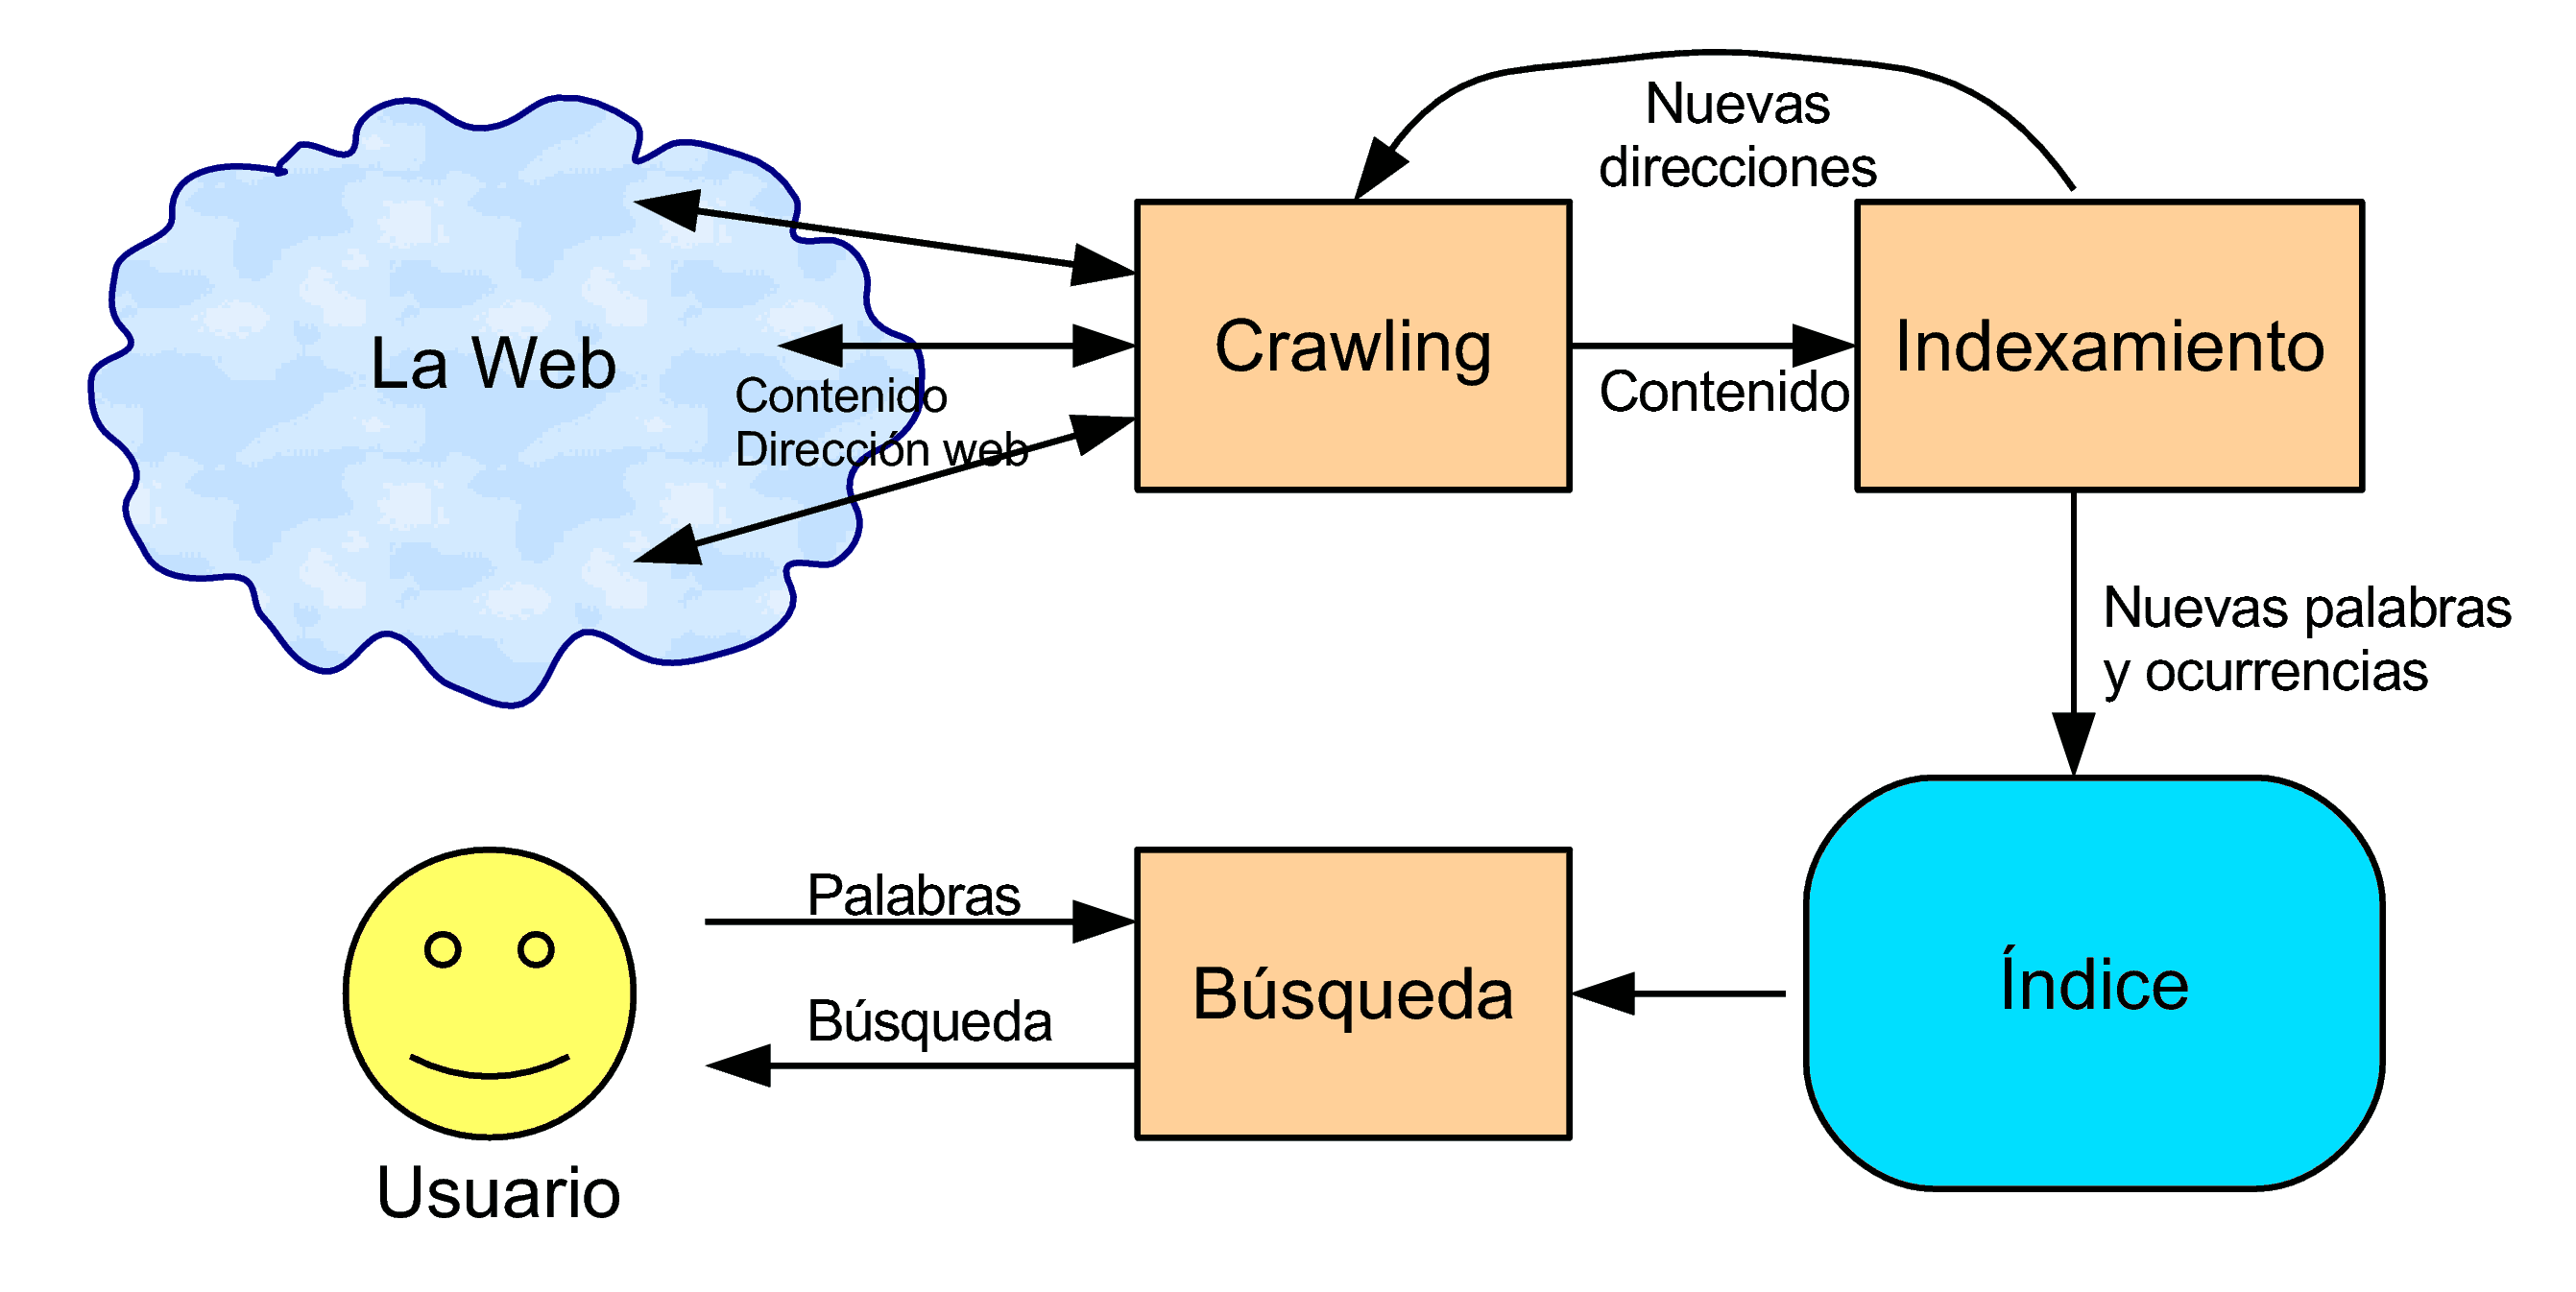
\includegraphics[scale=0.11]{pics/searchengine.png}
	\caption{ Diagrama Motor de Búsqueda ~\cite{libroweb2008}.}
\end{figure}

\end{frame}

\begin{frame}\frametitle{Modelo Vectorial}
\footnotesize{
\begin{itemize}
 \item Para poder rankear las consultas, o medir la similitud entre dos documentos necesitamos una métrica de similitud.
 \item Representamos los documentos como vectores de términos, donde cada término es una dimensión.
 \item A este tipos de modelos se le llame \emph{Bag of Words}. Perdemos el orden de las palabras. 
 \item El valor de cada dimensión, es un peso que representa la relevancia del término $t_{i}$ en el documento $d$.

\begin{equation}
 d_{j} \rightarrow \overrightarrow{d_{j}}=(w(t_{1},d_{j}),...,w(t_{|V|},d_{j}))
\end{equation}

\item ¿Cómo podemos modelar el aporte de información de un término en un documento?
 
\end{itemize}

}
 
\end{frame}

\begin{frame}\frametitle{Term Frecuency - Inverted Document Frecuency [1]}
\footnotesize{
\begin{itemize}
 \item Se define $Tf_{i,j}$, como la frecuencia del término $t_{i}$ en el documento $d_{j}$.
 \item Un término que aparece $10$ veces debiese aportar mayor información que uno aparece una vez.
 \item ¿Qué pasa cuando tenemos documentos muchos más largos que otros?
 \item Podemos normalizar por la frecuencia máxima de término en el documento. 
\begin{displaymath}
 Tf_{i,j}=\frac{f_{i,j}}{max \ f_{i,j}}
\end{displaymath}
\item ¿Un término que aparece en muy pocos documentos aporta más o menos información que uno que aparece varias veces?
\item Por ejemplo, el documento \emph{El señor alcalde de Malloco}. El término \emph{Malloco} aparece en menos documentos que \emph{alcalde}, por lo que debiese ser más descriptivo. 
\end{itemize}


} 
\end{frame}

\begin{frame}\frametitle{Term Frecuency - Inverted Document Frecuency [2]}
\footnotesize{ 
\begin{itemize}
 \item Sea $Q$ el número de documentos en la colección y $n_{i}$ el número de documentos donde aparece el término $t_{i}$, se define el $idf$ del término $t_{i}$ como: 
 \begin{displaymath}
  idf_{t_{i}}= log_{10}(\frac{Q}{n_{i}})
 \end{displaymath}
\item Un término que aparece en todos los documentos tendría $idf=0$ y uno que aparece en el $10\%$ de la colección tendría $idf=1$.

\item El modelo de score $Tf-idf$ combina ambos modelos, quedando el peso $w$ de un término sobre un documento como:
\begin{displaymath}
w(t_{i},d_{j})=Tf_{i}\times log_{10}(\frac{Q}{n_{i}}) 
\end{displaymath}

\item Las consultas a un motor de búsqueda también pueden modelarse como vectores, pero las consultas tienen en promedio entre $2$ y $3$ términos. Para evitar tener tantas dimensiones nulas, se usa un factor de suavizamiento en el vector:
\begin{displaymath}
 w(t_{i},d_{j})=(0.5+0.5\times Tf_{i,j})log_{10}(\frac{Q}{n_{i}}) 
\end{displaymath}



\end{itemize}



}

\end{frame}

\begin{frame}\frametitle{Similitud entre Vectores}
\footnotesize{
\begin{itemize}
 \item Una vez representados, los documentos y consultas como vectores, podemos medir su similitud.
 \item Una alternativa sería usar la distancia euclidiana, pero la variabilidad de largo entre documentos afectaría a la métrica.
 \item Lo más usado es usar el coseno del ángulo entre los vectores como medida de similitud.
 \item Si los documentos son iguales, el ángulo vale $0$ y el coseno $1$. En cambio si son ortogonales el coseno vale $0$.
 \item Los vectores, deben ser normalizados por su norma euclidiana $||d||_{2}$, la similitud de calcula de la siguiente manera:  
 \begin{displaymath}
 cos(d_{1},d_{2})= \frac{d_{1}\cdot d_{2}}{|d_{1}|\times|d_{2}|} = \frac{\sum_{i=1}^{|V|}(w(t_{i},d_{1})\times w(t_{i},d_{1}))}{\sqrt{\sum_{i=1}^{|V|} w(t_{i},d_{1})^2}\times \sqrt{\sum_{i=1}^{|V|} w(t_{i},d_{2})^2}}
\end{displaymath}
\item Erróneamente se llama \emph{distancia coseno}, realmente es una medida de similitud.


\end{itemize}


}
\end{frame}

\begin{frame}{Similitud Coseno}

\begin{figure}[h!]
	\centering
	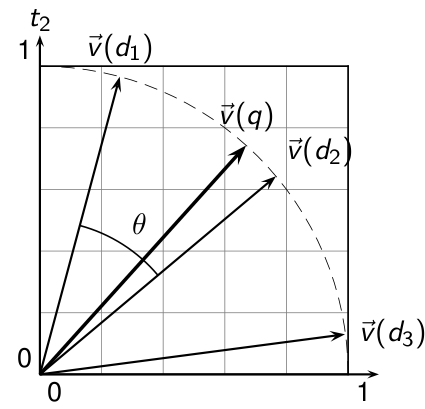
\includegraphics[scale=0.5]{pics/cos.png}
	\caption{ Similitud coseno.}
\end{figure}

\end{frame}

\begin{frame}{Ejercicio}
\begin{itemize}
 \item Supongamos que tenemos $3$ documentos, los cuales se forman a partir de las siguientes secuencias de términos: \\
 $d_{1}\rightarrow t_{4}t_{3}t_{1}t_{4}$ \\
 $d_{2}\rightarrow t_{5}t_{4}t_{2}t_{3}t_{5}$ \\
 $d_{3}\rightarrow t_{2}t_{1}t_{4}t_{4}$ \\

\item Construya una matriz término-documento de dimensión $5 \times 3$ usando los pesos $Tf-idf$ simples (sin normalización).
\item Le recomendamos construir primero una lista con la cantidad de documentos en los que aparece cada término (para el idf) 
\item Calcule luego  el $idf$ de cada término.
\item Llene las celdas con los valores $Tf-idf$
\item ¿ A qué documento está más cercano $d_{1}$?
\end{itemize}


\end{frame}

\begin{frame}{Resultado}
 \begin{table}[htbp]
\caption{Matriz Tf-idf}
\begin{tabular}{|l|r|r|r|}
\hline
 & \multicolumn{1}{l|}{d1} & \multicolumn{1}{l|}{d2} & \multicolumn{1}{l|}{d3} \\ \hline
t1 & 0.176 & 0.000 & 0.176 \\ \hline
t2 & 0.000 & 0.176 & 0.176 \\ \hline
t3 & 0.176 & 0.176 & 0.000 \\ \hline
t4 & 0.000 & 0.000 & 0.000 \\ \hline
t5 & 0.000 & 0.954 & 0.000 \\ \hline
\end{tabular}
\end{table}

\end{frame}

\begin{frame}{Clustering de Documentos [1]}
\footnotesize{
\begin{itemize}
 \item ¿Qué pasa si queremos agrupar los documentos de contenidos similares?
 \item Agrupamos los documentos en conjuntos, donde todos los elementos sean similares entre sí. 
 \item A cada conjunto se le llama  \emph{cluster}. 
 \item El problema de clusterizar, se basa en identificar grupos que maximicen la similitud interna dentro de un cluster y minimicen la similitud entre documentos  pertenecientes a distintos clusters ~\cite{adaptivewebsites}.
\begin{figure}[h!]
	\centering
	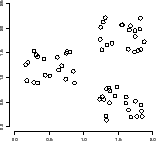
\includegraphics[scale=0.6]{pics/cluster.png}
	\caption{ Conjunto de documentos donde se identifica claramente cada cluster}
\end{figure}
 
\end{itemize}


}
 
\end{frame}

\begin{frame}{Clustering de Documentos [2]}
\footnotesize{
\begin{itemize}
 \item Permite identificar grupos de opiniones similares, o reducir el espacio de búsqueda para una consulta en un buscador. 
 \item K-medias es un algoritmo simple de clustering que requiere la cantidad $k$ de clusters a construir como parámetro.
    \begin{enumerate}
    \footnotesize{
    \item Primero, se identifican aleatoriamente $k$ elementos. Los valores de los atributos de éstos elementos se copian en nuevos elementos llamados centroides de la misma dimensión que éstos. Cada centroide representará un cluster.
    \item Luego se calcula la distancia de todos los $n$ elementos a los $k$ centroides y  se asigna  cada elemento al cluster del centroide más cercano.
    \item Luego se recalcula el valor de los centroides promediando el valor de los atributos de todos los elementos pertenecientes al cluster.
    \item Repite el proceso de calcular las distancias, agrupar los más cercanos y recalcular los centroides hasta que éstos dejen de cambiar. }
    \end{enumerate}

\end{itemize}
}
\end{frame}

\begin{frame}{K-medias}
\begin{figure}[h!]
	\centering
	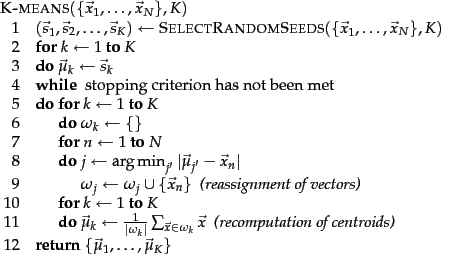
\includegraphics[scale=0.6]{pics/kmeans.png}
	\caption{ Algoritmo K-medias}
\end{figure}


 



 
\end{frame}




\begin{frame}[allowframebreaks]\scriptsize
\frametitle{References}
\bibliography{bio}
\bibliographystyle{apalike}
%\bibliographystyle{flexbib}
\end{frame}



%%%%%%%%%%%%%%%%%%%%%%%%%%%

\end{document}
